%======================================================================
\chapter{Formal Verification with Scyther}
\label{ch:scyther}
%======================================================================

Arguing informally that a protocol is secure is unreliable; the Needham--Schroeder
public-key protocol was believed correct for seventeen years before Lowe found an attack on
it with a model checker \cite{lowe}. This chapter describes how we specified our protocol in
SPDL, why our first model failed, and what restructuring made all claims verify.

\section{What Scyther does}

Scyther \cite{scyther} takes a protocol description and a set of claims, and searches
exhaustively for a trace in which a Dolev--Yao adversary (Figure~\ref{fig:dolevyao})
violates a claim. Within its bound it either finds an attack and draws it, or returns a
proof of correctness. It reasons symbolically about unbounded numbers of concurrent
sessions, which is where subtle attacks live --- an adversary running two sessions in
parallel and relaying between them.

\section{Attempt 1: the monolithic model, and why it failed}

Our first specification mirrored the paper's presentation literally: one protocol,
\code{UWCFull}, with all five roles, symmetric keys \code{k(A,B)}, and nonces accumulating
along the chain.

\begin{lstlisting}[style=bad,caption={First attempt (commit \code{82d9b09}, since replaced).
Nonces from earlier hops are carried forward into later ones.}]
protocol UWCFull(UWS, SUB, BUOY, SAT, BS)
{
  role SUB {
    var Nu: Nonce;  fresh Ns: Nonce;  var Nb: Nonce;
    recv_1(UWS, SUB, {UWS, Nu}k(UWS,SUB));
    send_2(SUB, UWS, {SUB, UWS, Nu, Ns}k(UWS,SUB));
    send_3(SUB, BUOY, {SUB, UWS, Nu, Ns}k(SUB,BUOY));      /* Nu crosses the hop */
    recv_4(BUOY, SUB, {BUOY, SUB, UWS, Nu, Ns, Nb}k(SUB,BUOY));
    claim(SUB, Alive);  claim(SUB, Niagree);  claim(SUB, Secret, Ns);
  }
  /* ... BUOY, SAT, BS roles similarly accumulate every prior nonce ... */
}
\end{lstlisting}

Three problems followed from this shape.

\begin{enumerate}
\item \textbf{Nonces crossed hop boundaries.} $N_u$, generated by the sensor, appeared in
      messages between SUB and BUOY. This contradicts the base paper's own design ---
      Section~IV-C states explicitly that hop-wise freshness ``eliminates the need for
      end-to-end nonce propagation'' --- and it widens the exposure of every nonce to every
      downstream node.
\item \textbf{Agreement claims failed.} With five roles interleaved in one protocol,
      \code{Niagree} could not be established: the adversary can run partial sessions and
      recombine message fragments across roles, because nothing in the message content ties
      a fragment to the hop it belongs to.
\item \textbf{Symmetric keys \code{k(A,B)} misrepresented the protocol.} The paper uses
      public-key encryption under the recipient's key, not a pre-shared symmetric key.
\end{enumerate}

\section{Attempt 2: four independent NSL hops}

The rewrite applied one insight: \emph{the base protocol is not one five-party protocol, it
is four independent two-party protocols that happen to run in sequence}. Modelling it that
way is both more faithful and easier to verify.

Each hop was written as a \textbf{Needham--Schroeder--Lowe} exchange --- the classic
three-message mutual authentication, with Lowe's fix.

\begin{figure}[H]
\centering
\resizebox{\textwidth}{!}{%
\begin{tikzpicture}[x=1cm,y=1cm,font=\scriptsize]
%--------------- LEFT: old model
\node[font=\small\bfseries\sffamily,text=coral,anchor=west] at (0,1.0) {ATTEMPT 1 \textemdash\ one protocol, 5 roles};
\draw[draw=coral,rounded corners=2pt] (-0.3,-5.6) rectangle (6.6,0.6);
\foreach \y/\nm in {0/UWS, -1.1/SUB, -2.2/BUOY, -3.3/SAT, -4.4/BS}
  {\node[box,anchor=west,minimum width=17mm,fill=white] at (0.1,\y) {\nm};}
\draw[flow,draw=coral] (2.0,0) -- (2.0,-1.1);
\draw[flow,draw=coral] (2.4,-1.1) -- (2.4,-2.2);
\draw[flow,draw=coral] (2.8,-2.2) -- (2.8,-3.3);
\draw[flow,draw=coral] (3.2,-3.3) -- (3.2,-4.4);
\draw[->,draw=coral,thick,dashed] (2.05,-0.15) .. controls (5.4,-0.9) and (5.4,-1.6) .. (2.45,-2.05);
\draw[->,draw=coral,thick,dashed] (2.45,-1.25) .. controls (6.0,-2.0) and (6.0,-2.8) .. (2.85,-3.15);
\node[font=\tiny,text=coral,anchor=west,align=left] at (3.6,-4.9)
  {dashed: $N_u$ and $N_s$ propagate\\ into hops they do not belong to};
\node[box,anchor=west,fill=palecoral,draw=coral,align=left,minimum width=58mm,font=\tiny] at (-0.2,-6.4)
  {\textbf{\textcolor{coral}{Result:}} \code{Niagree} fails. The adversary interleaves partial\\
   runs of different roles; nothing binds a message to its hop.};
%--------------- RIGHT: new model
\node[font=\small\bfseries\sffamily,text=kelp,anchor=west] at (8.4,1.0) {ATTEMPT 2 \textemdash\ four independent protocols};
\draw[draw=kelp,rounded corners=2pt] (8.1,-5.6) rectangle (16.0,0.6);
\foreach \y/\nm/\a/\b in {0/uwchop1/UWS/SUB, -1.4/uwchop2/SUB/BUOY,
                          -2.8/uwchop3/BUOY/SAT, -4.2/uwchop4/SAT/BS}
 {\node[box,anchor=west,minimum width=68mm,align=left,fill=mist,draw=kelp] at (8.4,\y)
   {\textbf{\code{\nm}}\ \ \ \a\ $\leftrightarrow$\ \b \ \ \textemdash\ \ own nonces, own tags, 8 claims};}
\node[box,anchor=west,fill=palekelp,draw=kelp,align=left,minimum width=66mm,font=\tiny] at (8.3,-6.4)
  {\textbf{\textcolor{kelp}{Result:}} 32/32 claims Ok, no attacks, 0.19\,s at max-runs 5.\\
   Faithful to the paper's hop-wise freshness design.};
\end{tikzpicture}}
\caption[Restructuring the Scyther model]{\textbf{The change that made verification
succeed.} Splitting one five-role protocol into four independent two-role protocols removes
cross-hop nonce propagation, matches the base paper's stated design, and lets Scyther prove
each hop in isolation. The claim count rises from 15 to 32 because each hop now carries a
full set of four claims per role.}
\label{fig:scyther-restructure}
\end{figure}

\subsection{The Needham--Schroeder--Lowe pattern}

Each hop is three messages:
\begin{align}
\text{Initiator} \to \text{Responder}&: \ \{\mathrm{Tag}_a,\ \text{Initiator},\ N_i\}_{pk(\text{Responder})} \notag\\
\text{Responder} \to \text{Initiator}&: \ \{\mathrm{Tag}_b,\ N_i,\ N_r,\ \textbf{Responder}\}_{pk(\text{Initiator})} \notag\\
\text{Initiator} \to \text{Responder}&: \ \{\mathrm{Tag}_c,\ N_r\}_{pk(\text{Responder})} \notag
\end{align}

\begin{keybox}
\textbf{Lowe's fix, and why it is here.} The original 1978 Needham--Schroeder protocol
omitted the responder's identity from the second message. Lowe showed in 1996 \cite{lowe}
that this permits a man-in-the-middle: an adversary $I$, whom $A$ legitimately initiates a
session with, can relay $A$'s nonce into a fresh session with $B$, so that $B$ ends up
believing it is talking to $A$ while $A$ believes it is talking to $I$. Including the
responder's identity inside message~2 breaks the relay, because $A$ can see the reply came
from $I$ and not from $B$. Our specification includes it (\code{SUB} inside the \code{h1b}
message and so on), which is why \code{Niagree} holds.
\end{keybox}

\subsection{Message tags}

Each of the twelve modelled messages carries a distinct constant tag:

\begin{lstlisting}[style=good,caption={Tag declarations (\code{uwc\_protocol.spdl},
lines 16--20).}]
usertype Tag;
const h1a, h1b, h1c: Tag;      /* hop 1: UWS <-> SUB   */
const h2a, h2b, h2c: Tag;      /* hop 2: SUB <-> BUOY  */
const h3a, h3b, h3c: Tag;      /* hop 3: BUOY <-> SAT  */
const h4a, h4b, h4c: Tag;      /* hop 4: SAT <-> BS    */
\end{lstlisting}

Tags prevent \emph{type-flaw} and \emph{cross-protocol} confusion: without them, a message
from hop~2 has the same structural shape as a message from hop~1 and the adversary could
splice one into the other. With a tag inside the encryption, the two are distinguishable and
the splice fails.

\subsection{One hop in full}

\begin{lstlisting}[style=good,caption={Hop 1 of the verified specification
(\code{uwc\_protocol.spdl}, lines 22--54).}]
protocol uwchop1(UWS, SUB)
{
    role UWS
    {
        fresh Nu: Nonce;
        var   Ns: Nonce;

        send_1(UWS, SUB, {h1a, UWS, Nu}pk(SUB));
        recv_2(SUB, UWS, {h1b, Nu, Ns, SUB}pk(UWS));    /* SUB inside = Lowe's fix */
        send_3(UWS, SUB, {h1c, Ns}pk(SUB));

        claim(UWS, Alive);
        claim(UWS, Weakagree);
        claim(UWS, Niagree);
        claim(UWS, Secret, Nu);
    }

    role SUB
    {
        var   Nu: Nonce;
        fresh Ns: Nonce;

        recv_1(UWS, SUB, {h1a, UWS, Nu}pk(SUB));
        send_2(SUB, UWS, {h1b, Nu, Ns, SUB}pk(UWS));
        recv_3(UWS, SUB, {h1c, Ns}pk(SUB));

        claim(SUB, Alive);
        claim(SUB, Weakagree);
        claim(SUB, Niagree);
        claim(SUB, Secret, Ns);
    }
}
\end{lstlisting}

Hops 2, 3 and 4 are structurally identical with the roles and tags substituted:
\code{uwchop2(SUB, BUOY)}, \code{uwchop3(BUOY, SAT)}, \code{uwchop4(SAT, BS)}.

\section{Verification results}

Four protocols $\times$ two roles $\times$ four claims $=$ \textbf{32 claims}.

\begin{table}[H]
\centering
\caption{Verification run.}
\label{tab:verif-run}
\small
\begin{tabular}{@{}l l@{}}
\toprule
Tool & Scyther 1.3.0 (bundled in \code{scyther/scyther-w32-v1.3.0/})\\
Model & \code{uwc\_protocol.spdl}, 4 protocols, 8 roles\\
Bound & \code{--max-runs=5} (five concurrent sessions per role)\\
Adversary & Dolev--Yao\\
Runtime & 0.19\,s\\
\textbf{Result} & \textbf{32 of 32 claims Ok --- proof of correctness, zero attacks}\\
\bottomrule
\end{tabular}
\end{table}

\begin{table}[H]
\centering
\caption[Scyther claim results]{All 32 claims, by hop and role. Every cell is
\texttt{Ok [proof of correctness]}.}
\label{tab:claims-results}
\small
\begin{tabular}{@{}c l c c c c l c c c c@{}}
\toprule
\multirow{2}{*}{\textbf{Hop}} & \multicolumn{5}{c}{\textbf{Initiator}} &
\multicolumn{5}{c}{\textbf{Responder}}\\
\cmidrule(lr){2-6}\cmidrule(lr){7-11}
& Role & Aliv & Weak & Niag & Secr & Role & Aliv & Weak & Niag & Secr\\
\midrule
1 & UWS  & Ok & Ok & Ok & Ok ($N_u$)   & SUB  & Ok & Ok & Ok & Ok ($N_s$)\\
2 & SUB  & Ok & Ok & Ok & Ok ($N_s$)   & BUOY & Ok & Ok & Ok & Ok ($N_b$)\\
3 & BUOY & Ok & Ok & Ok & Ok ($N_b$)   & SAT  & Ok & Ok & Ok & Ok ($N_{sat}$)\\
4 & SAT  & Ok & Ok & Ok & Ok ($N_{sat}$) & BS & Ok & Ok & Ok & Ok ($N_{bs}$)\\
\bottomrule
\end{tabular}
\end{table}

\begin{figure}[H]
\centering
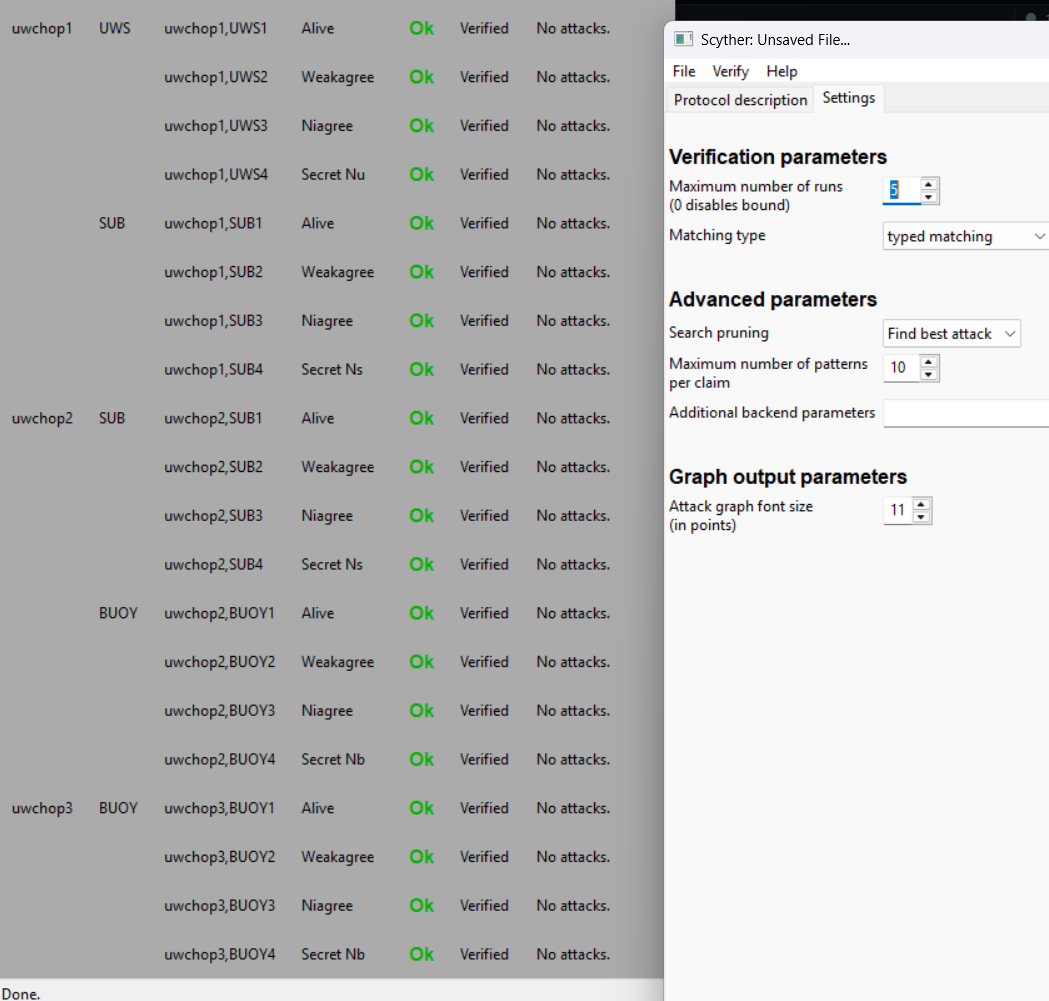
\includegraphics[width=0.95\textwidth]{figures/main-output.png}
\caption[Scyther GUI verification output]{\textbf{Scyther GUI output.} All 32 claims report
\texttt{Ok} with a proof of correctness. Reproduce with
\code{.\textbackslash Scyther\textbackslash scyther-w32.exe -{}-max-runs=5
..\textbackslash..\textbackslash uwc\_protocol.spdl}, or through the bundled GUI via
\code{launch\_scyther\_gui.bat}.}
\label{fig:scyther-gui}
\end{figure}

\section{Reading the result correctly}

\begin{warnbox}
\textbf{What 32/32 does and does not prove.} Scyther verifies the \emph{message design}
under the assumption of perfect cryptography. It proves that no ordering, interleaving,
replay or injection of messages by a Dolev--Yao adversary lets her learn a nonce or make a
node believe it authenticated someone it did not.

It does \emph{not} prove that AES-256-GCM is unbroken, that our Python is free of bugs, that
the random number generator is sound, or that a node's private key cannot be read out of
physical memory. Those are separate assurances --- respectively cryptanalysis,
implementation review, entropy sourcing, and the tamper-resistant storage the base paper
discusses in its Section~IV-E. Formal verification closes one class of vulnerability
completely and says nothing about the others.
\end{warnbox}

\section{Attacks addressed, and by what}

\begin{table}[H]
\centering
\caption{Attack coverage across the whole system.}
\label{tab:attacks}
\small
\begin{tabularx}{\textwidth}{@{}L{34mm} X L{34mm}@{}}
\toprule
\textbf{Attack} & \textbf{Defence} & \textbf{Established by}\\
\midrule
Replay & Fresh nonce per hop plus $|\Delta \TS| < 5$\,s & Simulation + Scyther
  (\code{Niagree})\\
Man-in-the-middle & ECDH under the recipient's public key; responder identity inside
  message~2 & Scyther (\code{Weakagree}, \code{Niagree})\\
Impersonation & $\ID = H(\PU)$ is unforgeable without the key pair & BAN logic (P1)\\
Eavesdropping & AES-256-GCM ciphertext over an ECDH-derived key & Scyther (\code{Secret})\\
Message tampering & 128-bit GHASH tag; decryption raises on mismatch & Cryptographic
  property of GCM\\
Node compromise & Ephemeral session keys plus BS revocation list & BAN logic (P5)\\
Delay injection & $z$-score outlier detection on the delay stream & Simulation (new in this
  project)\\
Cross-hop message splicing & Distinct tag constant inside every message & Scyther (all
  claims)\\
\bottomrule
\end{tabularx}
\end{table}

\section{Reproducing the verification}

\begin{lstlisting}[style=plain,caption={Command-line verification.}]
cd scyther/scyther-w32-v1.3.0
.\Scyther\scyther-w32.exe --max-runs=5 ..\..\uwc_protocol.spdl
\end{lstlisting}

Expected output: 32 lines, each ending \code{Ok [proof of correctness]}, in under one
second. For the GUI, run \code{launch\_scyther\_gui.bat} from the project root, open
\code{uwc\_protocol.spdl}, set max-runs to 5, and press Verify. The GUI additionally needs
\code{wxPython} and Graphviz on the system PATH.
